\documentclass[border=3pt,tikz]{standalone}
\usepackage[utf8]{vietnam}
\usetikzlibrary{calc,angles,intersections,shapes.geometric,arrows,decorations.markings,arrows.meta,patterns.meta,patterns}
\usepackage{tikz-3dplot,pgfplots}
\pgfplotsset{compat=1.15}
\usepgfplotslibrary{polar}
\usepackage{amsmath}
\begin{document}
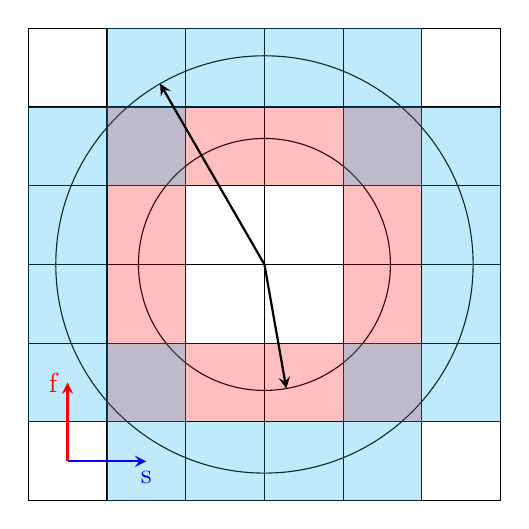
\begin{tikzpicture}[declare function={R=2.65;r=1.6;}]
	\draw (-3,-3) grid (3,3);
\path[draw, name path=dtr1] circle (r);
\path[draw, name path=dtr2] circle (R);
\foreach \y in {-3,...,2} {
	\foreach \x in {-3,...,2} {
		\path[name path=s-\x-\y] (\y,\x) rectangle ({\y+1},{\x+1});
		\path[name intersections={of=dtr1 and s-\x-\y, total=\t}]
		\pgfextra{\xdef\interseccount{\t}};
		\ifnum\interseccount>0\relax
		\fill[red, opacity=.25] (\y,\x) rectangle ({\y+1},{\x+1});
		\fi
		\path[name intersections={of=dtr2 and s-\x-\y, total=\s}]
		\pgfextra{\xdef\interseccounts{\s}};
		\ifnum\interseccounts>0\relax
		\fill[cyan, opacity=.25] (\y,\x) rectangle ({\y+1},{\x+1});
		\fi
	}
}
\draw[-stealth,thick] (0,0)--(120:R);
\draw[-stealth,thick] (0,0)--(-80:r);
\draw[-stealth,red,thick] (-2.5,-2.5)--+(90:1) node[left]{f};
\draw[-stealth,blue,thick] (-2.5,-2.5)--+(0:1) node[below]{s};
\end{tikzpicture}
\end{document}